% !TeX encoding = UTF-8

% 载入 SJTUThesis 模版
\documentclass[type=bachelor,oneside]{sjtuthesis}
% 选项
%   type=[doctor|master|bachelor],     % 可选(默认:master),论文类型
%   zihao=[-4|5],                      % 可选(默认:-4),正文字号大小
%   lang=[zh|en|de|ja],                % 可选(默认:zh),论文的主要语言
%   review,                            % 可选(默认:关闭),盲审模式
%   [twoside|oneside],                 % 可选(默认:twoside),双页或单页边距模式
%   [openright|openany],               % 可选(默认:openright),奇数页或任意页开始新章
%   math-style=[ISO|TeX],              % 可选 (默认:ISO),数学符号样式
\usepackage[hidelinks]{hyperref}


% 论文基本配置,加载宏包等全局配置
% !TEX root = ./main.tex

\sjtusetup{
  %
  %******************************
  % 注意:
  %   1. 配置里面不要出现空行
  %   2. 不需要的配置信息可以删除
  %******************************
  %
  % 信息录入
  %
  info = {%
    %
    % 标题
    %
    zh / title           = {颗粒介质中的超声波传播},
    en / title           = {Ultrasonic Propagation in Granular Media 
},
    %
    % 标题页标题
    %   可使用“\\”命令手动控制换行
    %
    % zh / display-title   = {上海交通大学学位论文\\ \LaTeX{} 模板示例文档},
    % en / display-title   = {A Sample Document \\ for \LaTeX-based SJTU Thesis Template},
    %
    % 关键词
    %
    zh / keywords        = {学位论文,论文格式,规范化,模板},
    en / keywords        = { dissertation, dissertation format, standardization, template},
    %
    % 姓名
    %
    zh / author          = {张三},
    en / author          = {\textbf{Zhang San}},
    %
    % 指导教师
    %
    zh / supervisor      = {李四},
    en / supervisor      = {\textbf{Li Si}},
    %
    % 副指导教师
    %
    % assoc-supervisor  = {某某教授},
    % assoc-supervisor* = {Prof. Uom Uom},
    %
    % 学号
    %
    id              = {520XXXXXXXX},
    %
    % 学位
    %   本科生不需要填写
    %
    zh / degree          = {学士},
    en / degree          = {Master of Engineering},
    %
    % 专业
    %
    zh / major           = {工业工程},
    en / major           = {A Very Important Major},
    %
    % 所属院系
    %
    zh / department      = {机械与动力工程学院},
    en / department      = {School of XXXXXXX},
    %
    % 答辩日期
    %   使用 ISO 格式 (yyyy-mm-dd);默认为当前时间
    %
     date                 = {2023-06},
    %
    % 标题页显示日期
    %   覆盖对应标题页的日期显示,原样输出
    %
     zh / display-date    = {20XX 年 XX 月},
    %
    % 资助基金
    %
    % zh / fund  = {
    %                {国家 973 项目 (No. 2025CB000000)},
    %                {国家自然科学基金 (No. 81120250000)},
    %              },
    % en / fund  = {
    %                {National Basic Research Program of China (Grant No. 2025CB000000)},
    %                {National Natural Science Foundation of China (Grant No. 81120250000)},
    %              },
  },
  %
  % 风格设置
  %
  style = {%
    %
    % 论文标题页 logo 颜色 (red/blue/black)
    %
    % title-logo-color = black,
  },
  %
  % 名称设置
  %
  name = {
    % bib             = {References},
    % ack             = {谢\hspace{\ccwd}辞},
    % achv            = {攻读学位期间完成的论文},
    digest={},
  },
}

% 使用 BibLaTeX 处理参考文献
%   biblatex-gb7714-2015 常用选项
%     gbnamefmt=lowercase     姓名大小写由输入信息确定
%     gbpub=false             禁用出版信息缺失处理
\usepackage[backend=biber,style=gb7714-2015]{biblatex}
% 文献表字体
% \renewcommand{\bibfont}{\zihao{5}\fixedlineskip{15.6bp}}
% 文献表条目间的间距
\setlength{\bibitemsep}{0pt}
% 导入参考文献数据库
\addbibresource{refs.bib}

% 脚注格式
\usepackage[perpage,bottom,hang]{footmisc}

% 定义图片文件目录与扩展名
\graphicspath{{figures/}}
\DeclareGraphicsExtensions{.pdf,.eps,.png,.jpg,.jpeg}

% 确定浮动对象的位置,可以使用 [H],强制将浮动对象放到这里(可能效果很差)
% \usepackage{float}

% 固定宽度的表格
% \usepackage{tabularx}

% 使用三线表:toprule,midrule,bottomrule。
\usepackage{booktabs}

% 表格中支持跨行
\usepackage{multirow}

% 表格中数字按小数点对齐
\usepackage{dcolumn}
\newcolumntype{d}[1]{D{.}{.}{#1}}

% 使用长表格
\usepackage{longtable}

% 附带脚注的表格
\usepackage{threeparttable}

% 附带脚注的长表格
\usepackage{threeparttablex}

% 算法环境宏包
\usepackage[ruled,vlined,linesnumbered]{algorithm2e}
% \usepackage{algorithm, algorithmicx, algpseudocode}

% 代码环境宏包
\usepackage{listings}
\lstdefinestyle{lstStyleCode}{%
  aboveskip         = \medskipamount,
  belowskip         = \medskipamount,
  basicstyle        = \ttfamily\zihao{6},
  commentstyle      = \slshape\color{black!60},
  stringstyle       = \color{green!40!black!100},
  keywordstyle      = \bfseries\color{blue!50!black},
  extendedchars     = false,
  upquote           = true,
  tabsize           = 2,
  showstringspaces  = false,
  xleftmargin       = 1em,
  xrightmargin      = 1em,
  breaklines        = false,
  framexleftmargin  = 1em,
  framexrightmargin = 1em,
  backgroundcolor   = \color{gray!10},
  columns           = flexible,
  keepspaces        = true,
  texcl             = true,
  mathescape        = true
}
\lstnewenvironment{codeblock}[1][]{%
  \lstset{style=lstStyleCode,#1}}{}

% 直立体数学符号
\providecommand{\dd}{\mathop{}\!\mathrm{d}}
\providecommand{\ee}{\mathrm{e}}
\providecommand{\ii}{\mathrm{i}}
\providecommand{\jj}{\mathrm{j}}

% 国际单位制宏包
\usepackage{siunitx}

% 定理环境宏包
\usepackage{ntheorem}
% \usepackage{amsthm}

% 绘图宏包
\usepackage{tikz}
\usetikzlibrary{arrows.meta, shapes.geometric}

% 一些文档中用到的 logo
\usepackage{hologo}
\providecommand{\XeTeX}{\hologo{XeTeX}}
\providecommand{\BibLaTeX}{\textsc{Bib}\LaTeX}

% 借用 ltxdoc 里面的几个命令方便写文档
\DeclareRobustCommand\cs[1]{\texttt{\char`\\#1}}
\providecommand\pkg[1]{{\sffamily#1}}

% hyperref 宏包在最后调用
\usepackage{hyperref}

% E-mail
\providecommand{\email}[1]{\href{mailto:#1}{\urlstyle{tt}\nolinkurl{#1}}}


\begin{document}
\setlength{\baselineskip}{20pt}

%TC:ignore

% 标题页
\maketitle

% 原创性声明及使用授权书
\copyrightpage
% 插入外置原创性声明及使用授权书
% 此时必须在导言区使用 \usepackage{pdfpages}
% \copyrightpage[scans/sample-copyright.pdf]

% 前置部分
\frontmatter
{
\fancyhead[LE,RO]{}
{
\ctexset{chapter={afterskip=26bp}}
% 摘要
% !TEX root = ../main.tex

\begin{abstract}[zh]
\addcontentsline{toc}{chapter}{摘 \quad 要}
  学位论文是本科生从事科研工作的成果的主要表现,集中表明了作者在研究工作中获得的新的发明、理论或见解,也是科研领域中的重要文献资料和社会的宝贵财富。
 \par 为了提高本科生学位论文的质量,做到学位论文在内容和格式上的规范化与统一化,特制作本模板。
\end{abstract}

{
\newfontface{\arial}{Arial}[Scale=0.94]
\ctexset{chapter/format+={\arial}}
\begin{abstract}[en]
\addcontentsline{toc}{chapter}{ABSTRACT}
As a primary means of demonstrating research findings for undergraduate students, dissertation is a systematic and standardized record of the new inventions, theories or insights obtained by the author in the research work. It can not only function as an important reference when students pursue further studies, but also contribute to scientific research and social development.
\par This template is therefore made to improve the quality of undergraduates’ dissertation and to further standardize it both in content and in format.

\end{abstract}
}
}

{
\ctexset{chapter={afterskip=26bp}}
\renewcommand{\cftchapfont}{\zihao{4}\bfseries}
\renewcommand{\cftsecfont}{\zihao{-4}}
\renewcommand{\cftsubsecfont}{\zihao{5}}
% 目录
\tableofcontents
}
}
% % 插图索引
% \listoffigures*
% % 表格索引
% \listoftables*
% % 算法索引
% \listofalgorithms*
% % 符号对照表
% \input{contents/nomenclature}

%TC:endignore

% 主体部分
\mainmatter

% 正文内容
{
\ctexset{chapter={afterskip=26bp}}
% !TEX root = ../main.tex

\chapter{绪论}

\section{引言}
学位论文……

\section{本文研究主要内容}
本文……

\section{本文研究意义}
本文……

\section{本章小结}
本文……


% !TEX root = ../main.tex

\chapter{正文文字格式}

\section{论文正文}
论文正文是主体,一般由标题、文字叙述、图、表格和公式等部分构成 \cite{Yang1999}。一般可包括理论分析、计算方法、实验装置和测试方法,经过整理加工的实验结果分析和讨论,与理论计算结果的比较以及本研究方法与已有研究方法的比较等,因学科性质不同可有所变化。
\par 论文内容一般应由十个主要部分组成,依次为:1.封面,2.中文摘要,3.英文摘要,4.目录,5.符号说明,6.论文正文,7.参考文献,8.附录,9.致谢,10.攻读学位期间发表的学术论文目录\cite{Yu2012}。
\par 以上各部分独立为一部分,每部分应从新的一页开始,且纸质论文应装订在论文的右侧。


\section{字数要求}
\subsection{本科论文要求}
各学科和学院自定。理工科研究类论文一般不少于2万字,设计类一般不少于1.5万字;医科、文科类论文一般不少于1万字。

\section{本章小结}
本章介绍了……


% !TEX root = ../main.tex

\chapter{图表、公式格式}

\section{图表格式}
\begin{figure}[!htp]
  \centering
  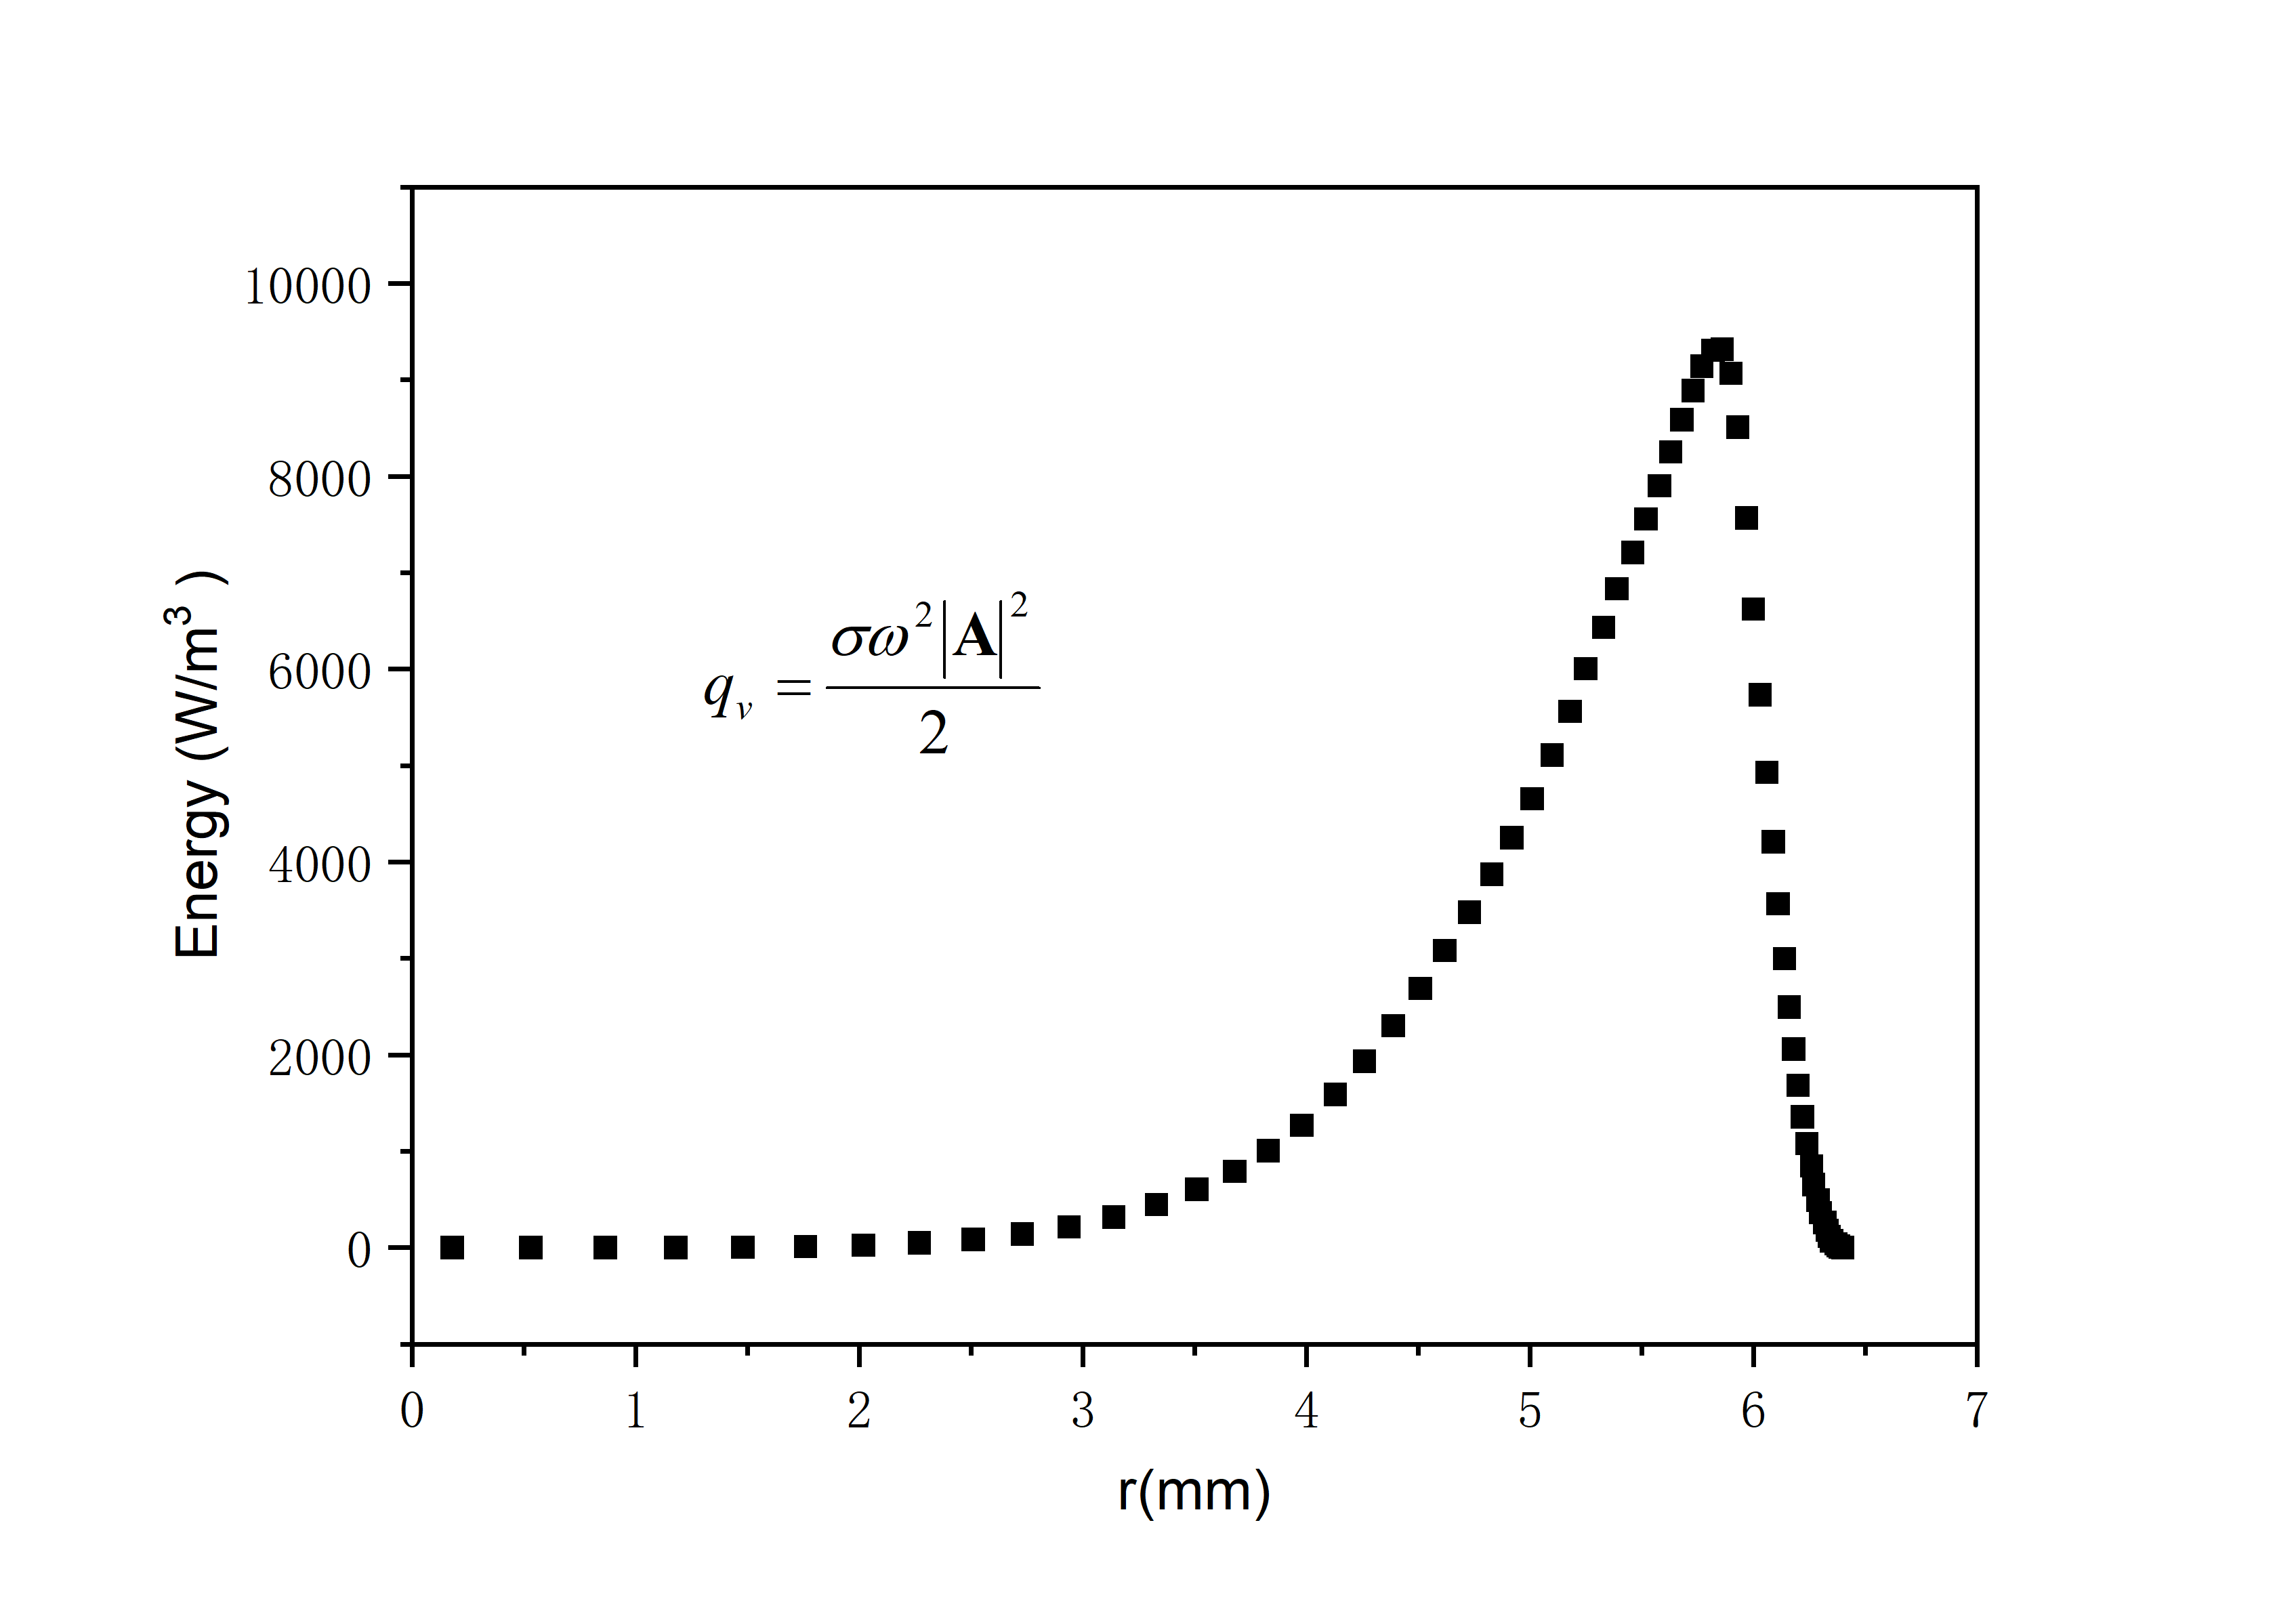
\includegraphics[width=8cm]{figures/energy.png} 
  \caption{内热源沿径向的分布}
  \label{fig:energy}
\end{figure}

\begin{figure}[!hbtp]
  \centering
  \subcaptionbox{健康/损伤信号}%
                [7cm]{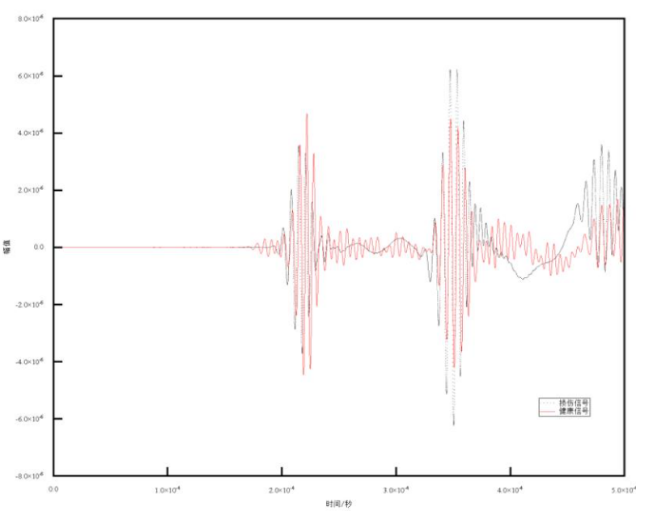
\includegraphics[height=6cm]{figures/signal_1.png}}
  \hspace{1cm}
  \subcaptionbox{散射信号}%
                [7cm]{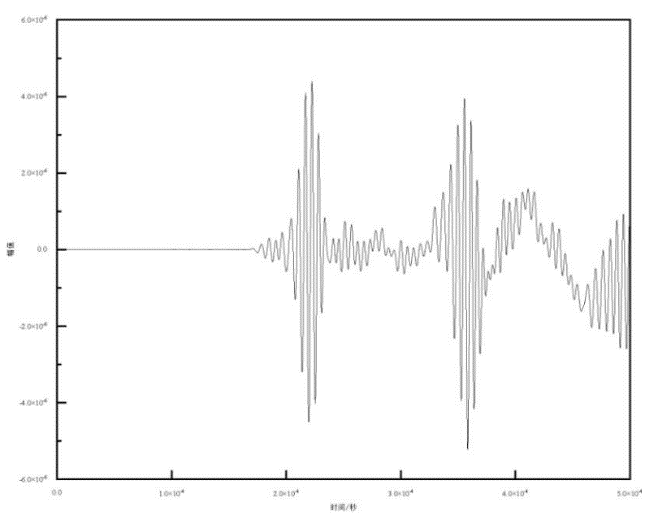
\includegraphics[height=6cm]{figures/signal_2.png}}
  \caption{响应信号处理}
  \label{fig:bisubcaptionbox}
\end{figure}

\begin{ThreePartTable}
  \begin{longtable}[c]{*{4}{c}}
    \caption{高频感应加热的基本参数}
    \label{tab:data} \\
    \toprule
     \multicolumn{1}{c}{感应频率} & \multicolumn{1}{c}{感应发生器功率}
      & \multicolumn{1}{c}{工件移动速度} & \multicolumn{1}{c}{感应圈与零件间隙}
    & \multicolumn{1}{c}{(kHz)} & \multicolumn{1}{c}{(\% ×80kW)}
    & \multicolumn{1}{c}{(mm/min)} & \multicolumn{1}{c}{(mm)}\\
    \midrule
    \endfirsthead
    \multicolumn{4}{l}{\textbf{续表~\thetable}} \\
    \toprule
     \multicolumn{1}{c}{感应频率} & \multicolumn{1}{c}{感应发生器功率}
      & \multicolumn{1}{c}{工件移动速度} & \multicolumn{1}{c}{感应圈与零件间隙}
    & \multicolumn{1}{c}{(kHz)} & \multicolumn{1}{c}{(\% ×80kW)}
    & \multicolumn{1}{c}{(mm/min)} & \multicolumn{1}{c}{(mm)}\\
    \midrule
    \endhead
    \hline
    \multicolumn{4}{r}{}
    \endfoot
    \endlastfoot
    250	& 88 & 5900	& 1.65 \\
    250	& 88 & 5900	& 1.65 \\
    250	& 88 & 5900	& 1.65 \\
    250	& 88 & 5900	& 1.65 \\
    250	& 88 & 5900	& 1.65 \\
    250	& 88 & 5900	& 1.65 \\
    250	& 88 & 5900	& 1.65 \\
    250	& 88 & 5900	& 1.65 \\
    250	& 88 & 5900	& 1.65 \\
    250	& 88 & 5900	& 1.65 \\
    250	& 88 & 5900	& 1.65 \\
    250	& 88 & 5900	& 1.65 \\
    250	& 88 & 5900	& 1.65 \\
    250	& 88 & 5900	& 1.65 \\
    250	& 88 & 5900	& 1.65 \\
    250	& 88 & 5900	& 1.65 \\
    250	& 88 & 5900	& 1.65 \\
    250	& 88 & 5900	& 1.65 \\
    250	& 88 & 5900	& 1.65 \\
    250	& 88 & 5900	& 1.65 \\
    250	& 88 & 5900	& 1.65 \\
    250	& 88 & 5900	& 1.65 \\
    250	& 88 & 5900	& 1.65 \\
    250	& 88 & 5900	& 1.65 \\
    250	& 88 & 5900	& 1.65 \\
    250	& 88 & 5900	& 1.65 \\
    250	& 88 & 5900	& 1.65 \\
    250	& 88 & 5900	& 1.65 \\
    250	& 88 & 5900	& 1.65 \\
    250	& 88 & 5900	& 1.65 \\
    250	& 88 & 5900	& 1.65 \\
    250	& 88 & 5900	& 1.65 \\
    250	& 88 & 5900	& 1.65 \\
    250	& 88 & 5900	& 1.65 \\
    250	& 88 & 5900	& 1.65 \\
    250	& 88 & 5900	& 1.65 \\
    250	& 88 & 5900	& 1.65 \\
    250	& 88 & 5900	& 1.65 \\
    250	& 88 & 5900	& 1.65 \\
    250	& 88 & 5900	& 1.65 \\
    250	& 88 & 5900	& 1.65 \\
    250	& 88 & 5900	& 1.65 \\
    250	& 88 & 5900	& 1.65 \\
    \bottomrule
  \end{longtable}
\end{ThreePartTable}

\section{公式格式}
\begin{equation}
 \frac{1}{\mu} \nabla^{2} \mathbf{A}-j \omega \sigma \mathbf{A}-\nabla\left(\frac{1}{\mu}\right) \times(\nabla \times \mathbf{A})+\mathbf{J}_{0}=0
\end{equation}


\section{本章小结}
本章介绍了……

% !TEX root = ../main.tex

\chapter{全文总结}


\section{主要结论}
本文主要\cite{Schinstock2000,Wen1990,Jiang1998,Fang2007,Zhang2012,GBT3792,Xiao2001}……

\section{研究展望}
更深入的研究……



}

%TC:ignore

\clearpage
{
\ExplSyntaxOn
\bool_if:NTF \g__sjtu_twoside_bool
{
    \fancyhead [ LE ]     { 参考文献 }
    \fancyhead [ RO ]     { 参考文献 }
}
{
    \fancyhead [ R ] { 参考文献 }
}
\ExplSyntaxOff
% 文献表字体
\renewcommand{\bibfont}{\zihao{5}}
% 设定固定间距
\fixedlineskip{15.6bp}
{
\ctexset{chapter={afterskip=26bp}}
% 参考文献
\printbibliography[heading=bibintoc]
}
\clearpage
}

\makeatletter
% \appendix采用数字编号。
\renewcommand{\appendix}{\par
    \setcounter{chapter}{0}
    \setcounter{section}{0}
    \ctexset{chapter/number={\arabic{chapter}}}
}
% 使用 \appchapter 替代附录中的 \chapter 章节,附录中的章节不再放入目录。
\newcommand{\appchapter}[1]{
    \refstepcounter{chapter}
    \SJTU@head*[附录 \thechapter]{#1(附录 \thechapter)}
}
\makeatother

{
\ctexset{chapter={afterskip=26bp}}
% 附录
\appendix
% 附录中图表不加入索引
\captionsetup{list=no}
% !TEX root = ../main.tex

\appchapter{符号与标记}\label{chap:symbol}
\addcontentsline{toc}{chapter}{附\quad 录}  

}


% 结尾部分
\backmatter

{
\ctexset{chapter={afterskip=26bp}}
% 发表论文及科研成果
% !TEX root = ../main.tex

\begin{achievements}

\begin{bibliolist}{00}
  \item 张三,李四. …… (已录用)
  
\end{bibliolist}


\end{achievements}

}

\clearpage
{
\ExplSyntaxOn
\bool_if:NTF \g__sjtu_twoside_bool
{
    \fancyhead [ LE ]     { 致谢 }
    \fancyhead [ RO ]     { 致谢 }
}
{
    \fancyhead [ R ] { 致谢 }
}
\ExplSyntaxOff
{
\ctexset{chapter={afterskip=26bp}}
% 致谢
% !TEX root = ../main.tex

\begin{acknowledgements}
 致谢主要感谢导师和对论文工作有直接贡献和帮助的人士和单位。致谢言语应谦虚诚恳,实事求是。
\end{acknowledgements}

}

\clearpage
}

{
\ctexset{chapter={afterskip=26bp}}
% 学士学位论文要求在最后有一个大摘要,单独编页码
% !TEX root = ../main.tex

\begin{digest}
  HCCI (Homogenous Charge Compression Ignition) combustion has advantages in terms of efficiency and reduced emission. HCCI combustion can not only ensure both the high economic and dynamic quality of the engine, but also efficiently reduce the NOx and smoke emission. Moreover, one of the remarkable characteristics of HCCI combustion is that the ignition and combustion process are controlled by the chemical kinetics, so the HCCI ignition time can vary significantly with the changes of engine configuration parameters and operating conditions. ……
\end{digest}

}

\end{document}
